\chapter{Experiment}
\label{ch:experiment}

In the Experiment an optical transmitter was simulated in OptSim. The Experiment was divided in three sub-projects.

\section{Project 1}
\label{sec:P1}

\begin{figure}[h]%
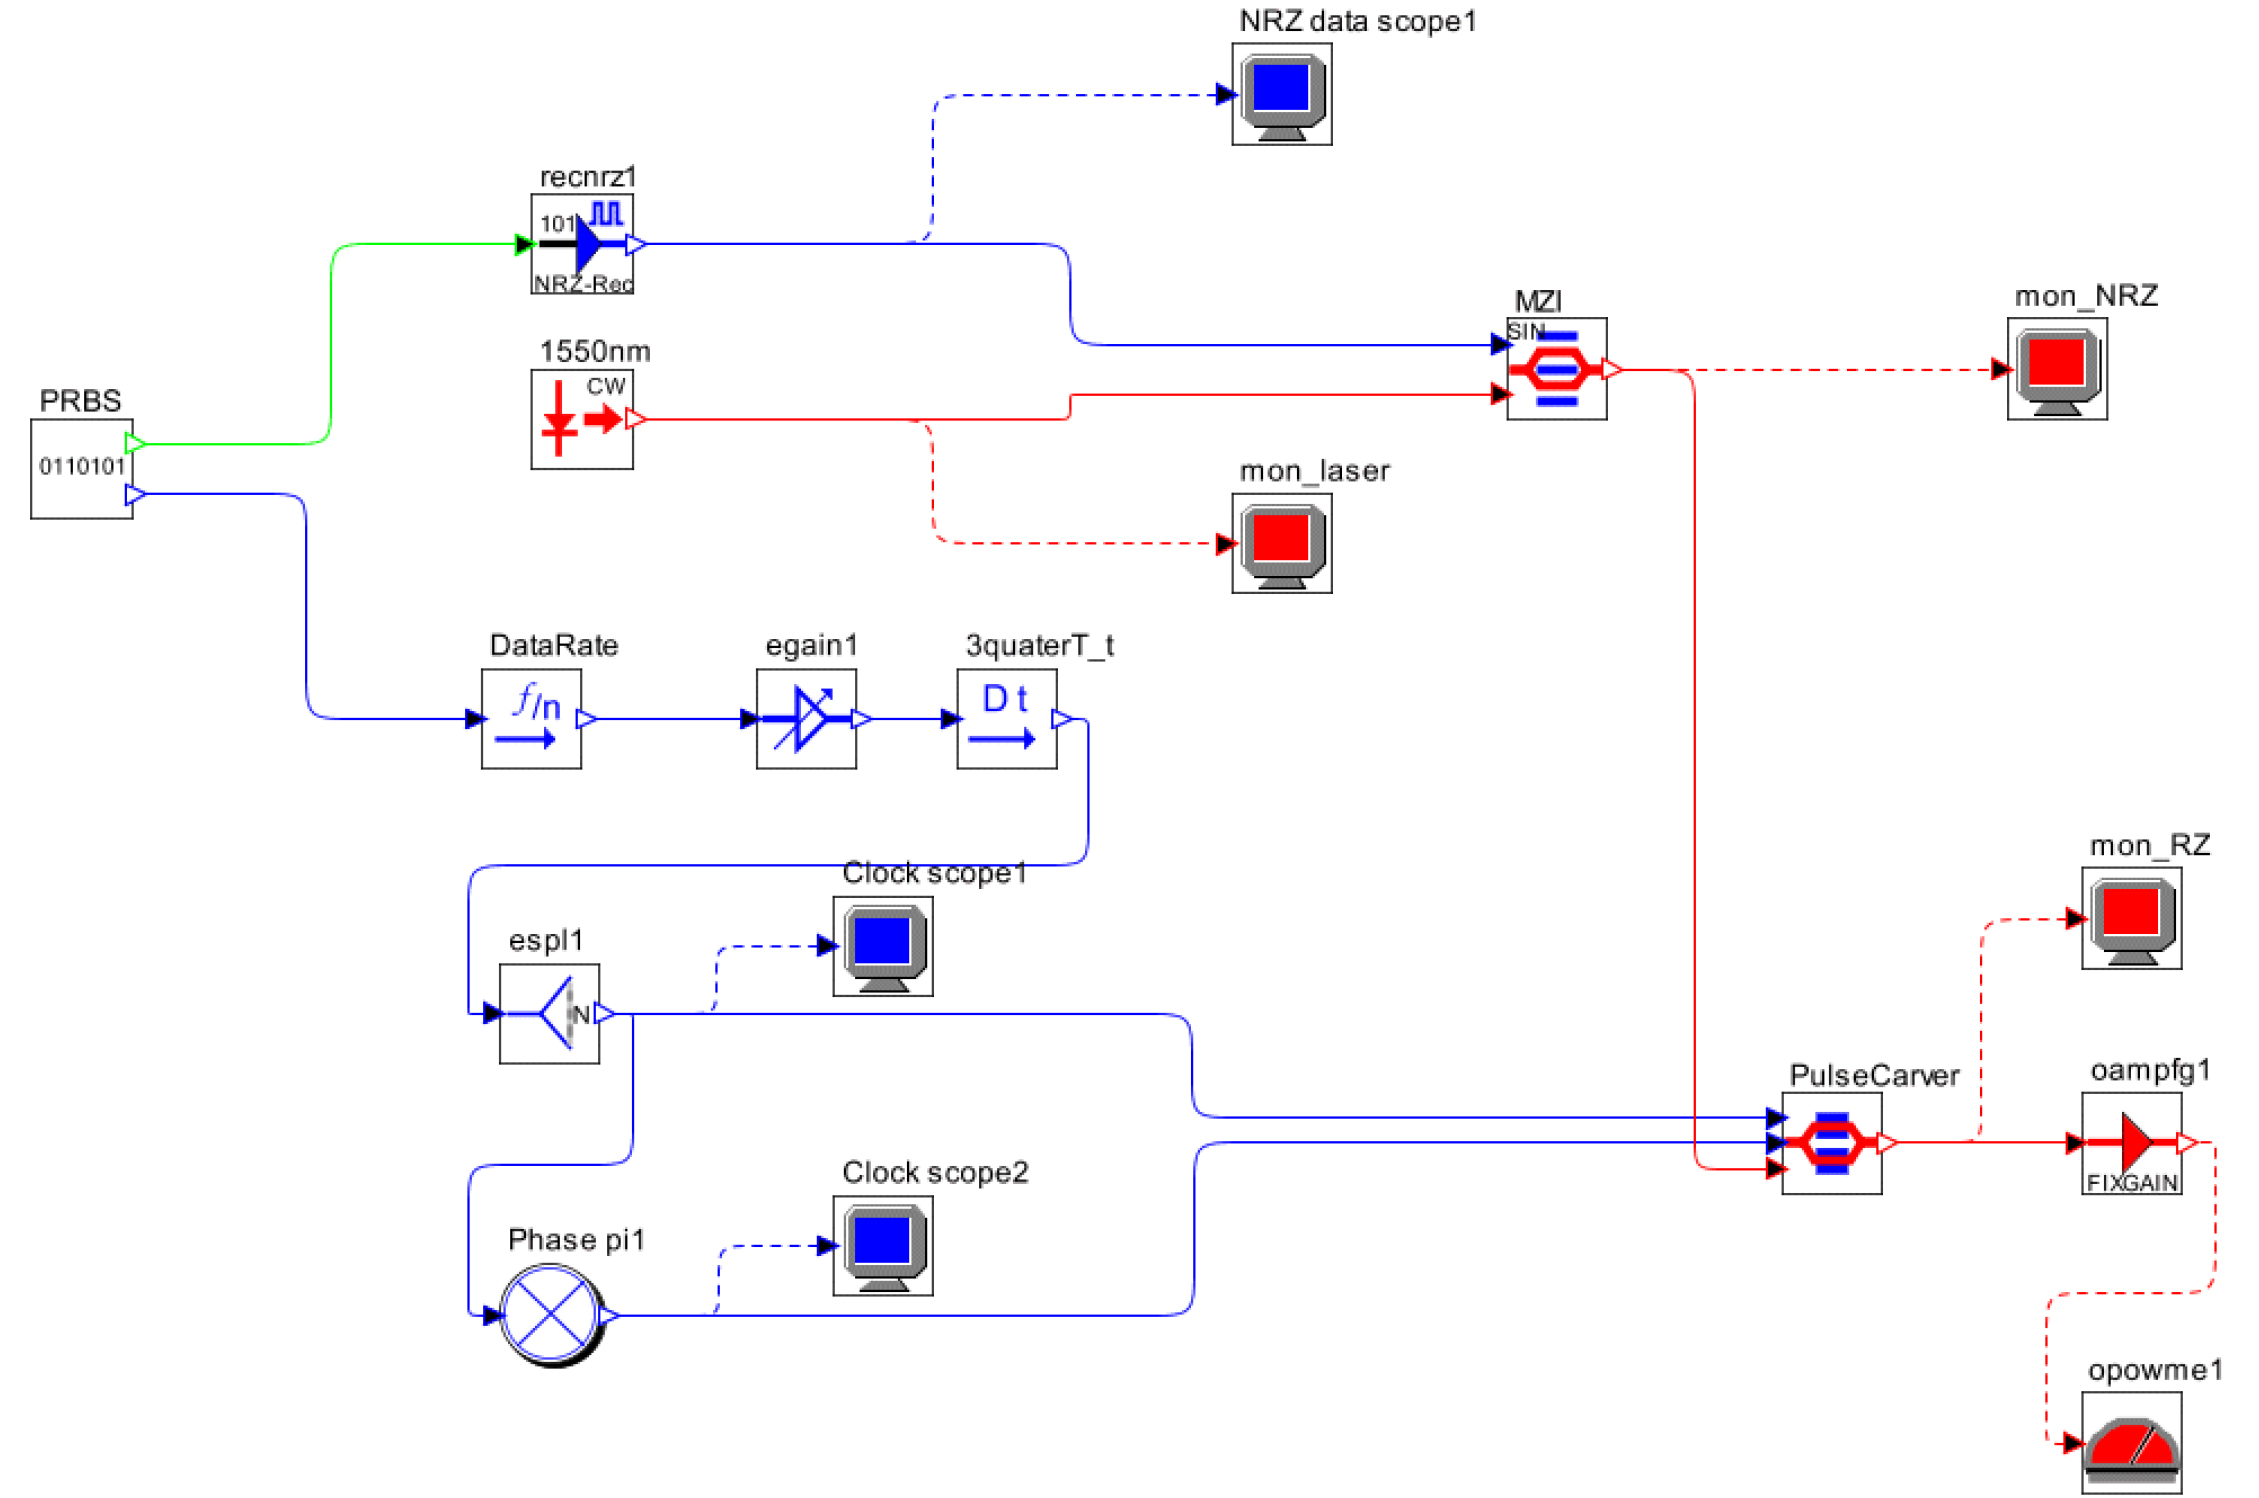
\includegraphics[width=.8\columnwidth]{Grafiken/P1_aufbau.jpg}%
\caption{Schematic: OptiSim Sample-Mode example of a 50~\% RZ-OOK-Transmitter}%
\label{fig:P1_aufbau}%
\end{figure}

For the Experiment an OptiSim Example of a 50~\% RZ-OOK-Transmitter was used. Figure \ref{fig:P1_aufbau} shows the schematic of this example\footnotemark[3]. In the upper left-hand side theres the PRBS which generates a pseudo-random bit-stream. A logical connection path (green) leads to an NRZ-Rectifier (recnrz1) which generates an electrical output signal. Via an MZI this electrical NRZ-signal gets modulated on a 1550~nm laser. 

Starting in the upper left-hand side at the PRBS again, the lower path leads to an divider. Here the DataRate can be divided. In the first project there is no change of the data rate and the divider is 1. Afer that there is an amplifier (egain1) and a time-delay element. Those elements are used to set the driving-voltage for the MZM (PulseCarver).

For driving the MZ in "`puhs-pull"' mode (cf. \ref{sec:MZM}) the phase of one electrical paths is shifted. The folloing MZM (PulseCarver) is used to carve the NRZ pulses to a NRZ-OOK signal.



\footnote[3]{Materials for the Preparation of Experiment 7: Simulation of Optical Transmitters}

Figure \ref{fig:P1ExB_Spectra} shows the spectrum of the laser source (red) and the spectrum of the optical NRZ signal (green). At a frequency of $f~\approx~193.415$~THz both spectra show a large peak. This is the laser frequency and therefor also the carrier frequency of the NRZ-Signal. 10~GHz beside the carrier frequency are the peaks of the 10~Gbit/s NRZ signal and it's harmonics. 

\begin{figure}%
\centering
%\begin{adjustwidth}{0cm}{0cm}
	\subfloat[Spectra]{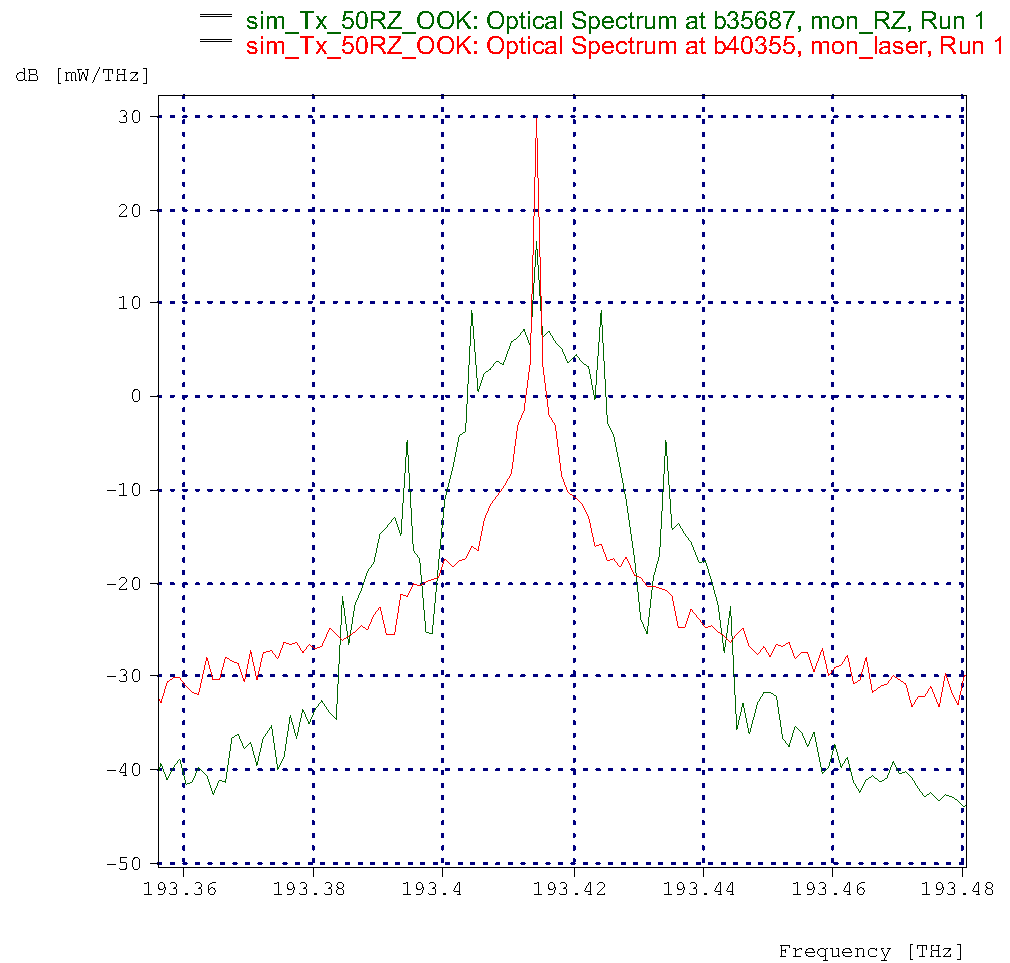
\includegraphics[totalheight=6 cm]{Grafiken/P1ExB_Spectra.pdf}\label{fig:P1ExB_Spectra}~}
	\subfloat[Eye Diagramm]{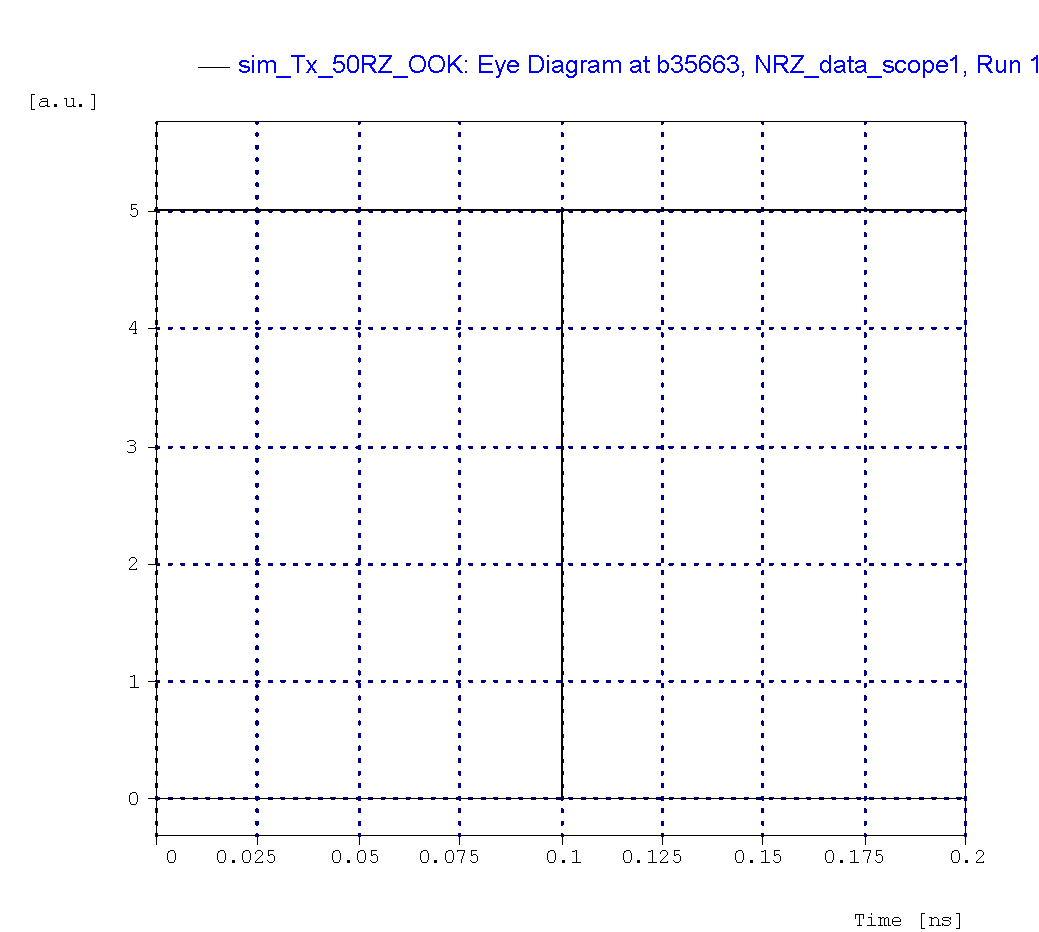
\includegraphics[totalheight=6 cm]{Grafiken/P1ExB_Eye.pdf} \label{fig:P1ExB_Eye}}%
%\end{adjustwidth}
\caption{\textbf{a)} Spectrum of the laser source (red) and spectrum of the NRZ-signal (green). \textbf{b)} Eye diagramm of the NRZ signal.}%
\label{fig:P1ExB_1}%
\end{figure}

Figure \ref{fig:P1ExB_Eye} shows an eye diagramm of the generated NRZ signal. 
\todo{Was bedeutet das? Was kann man hier sehen? WTF?} The measured log Q factor of the NRZ signal is 40 dB.

Taking a look at the electrical and the optical bit sequence shows, that they are matching (cf. \ref{fig:P1ExB_bit}).

\begin{figure}%
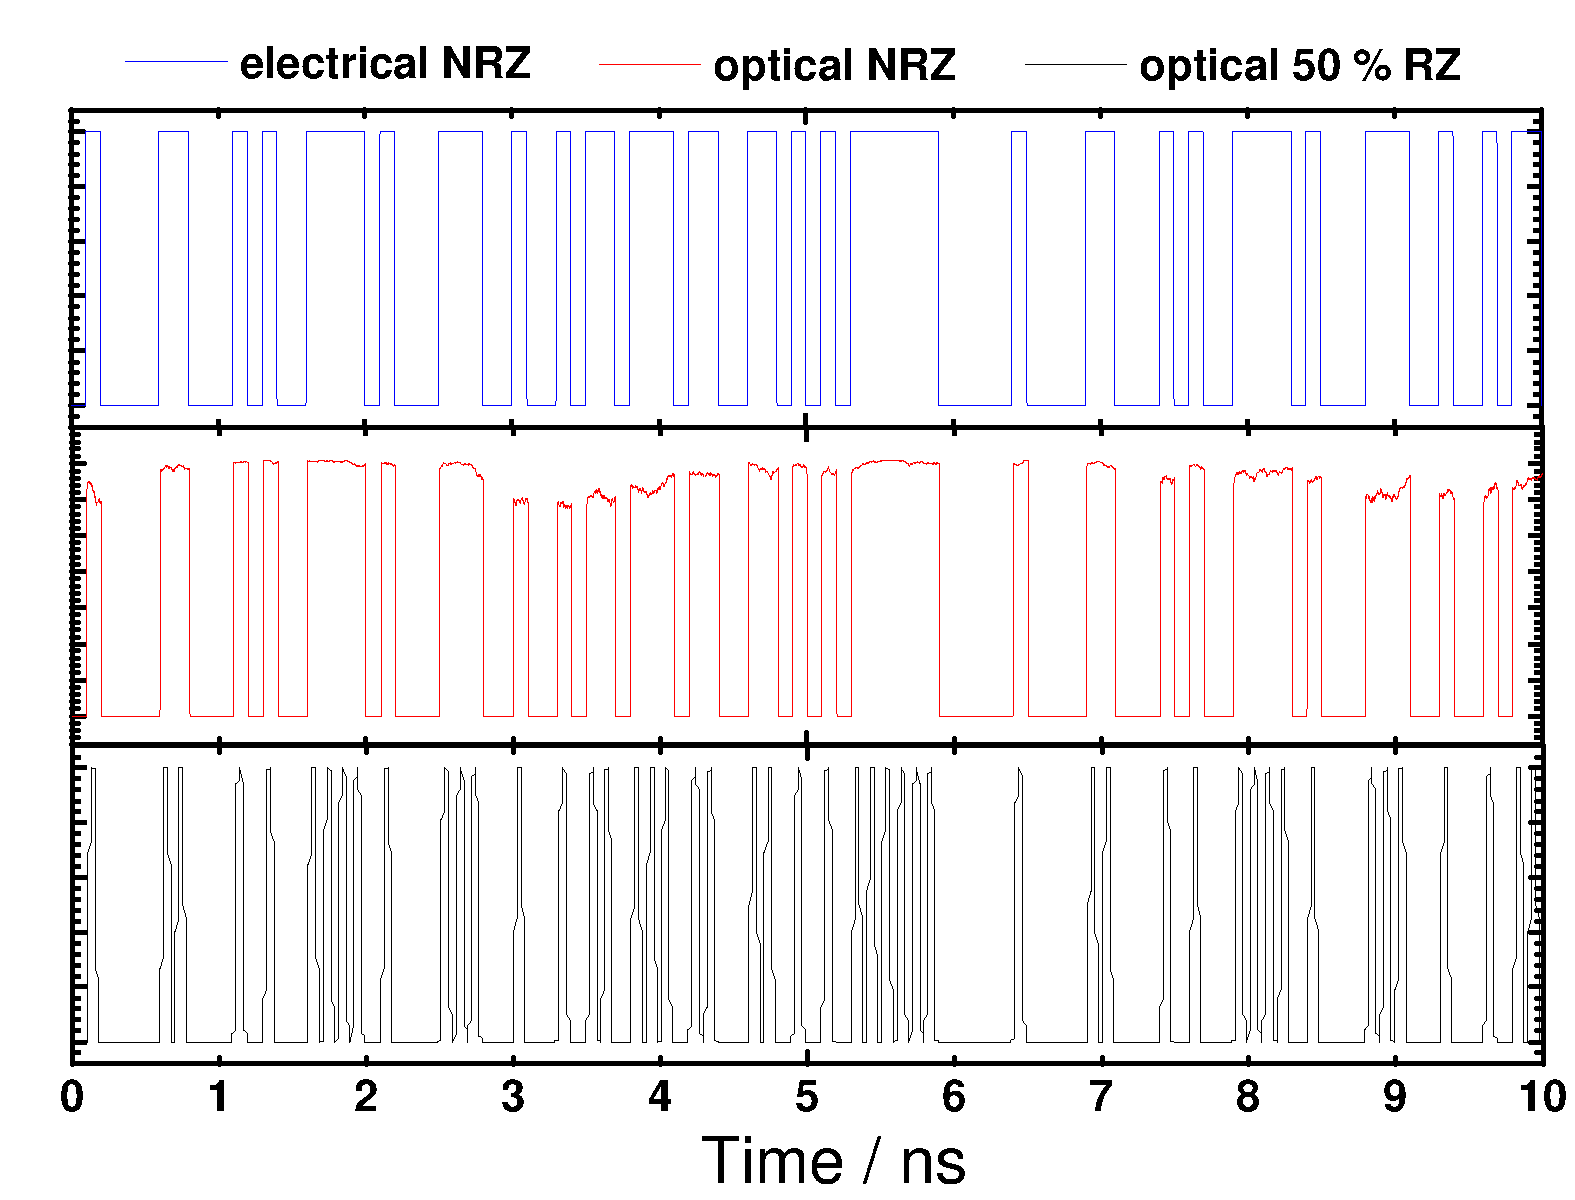
\includegraphics[width=\columnwidth]{Grafiken/P1ExB_BitSequence.pdf}%
\caption{NRZ bit sequences.}%
\label{fig:P1ExB_bit}%
\end{figure}